\section{Lecture 1: Blackbody Radiation}

\subsection{What is Physics?}

Why do we need quantum mechanics? \textcolor{red}{The older (classical) theory was wrong!}

Physics doesn't tell you ``why'' things work--it tells you ``how'' things work. The reality is not observable, quantum mechanics ``describes'' observations
rather than helping you ``understand'' some. By throwing away our philosophical concerns, we instead directly study the mathematics.

\subsection{The Potter's Problem: Blackbody Radiation}

Take a cube of some solid and heat it up to some temperature $T$. When you do this, it emits light (it glows). For a long time,
no one knew how this phenomenon worked. Here are some observations throw the ages:

\begin{itemize}
    \item 1792: Wedgewood notes that all objects (at a certain $T$) glow the same color.
    \item 1800s: With improvements in spectroscopy, we can now measure the frequency content of light.
    \item 1859: Kirchoff proposes a model. $R$ is the ``emissive power/area'', $\lambda$ is wavelength of the light and $T$ is the temperature.
    \[ R(\lambda, T) \]
    \begin{center}
    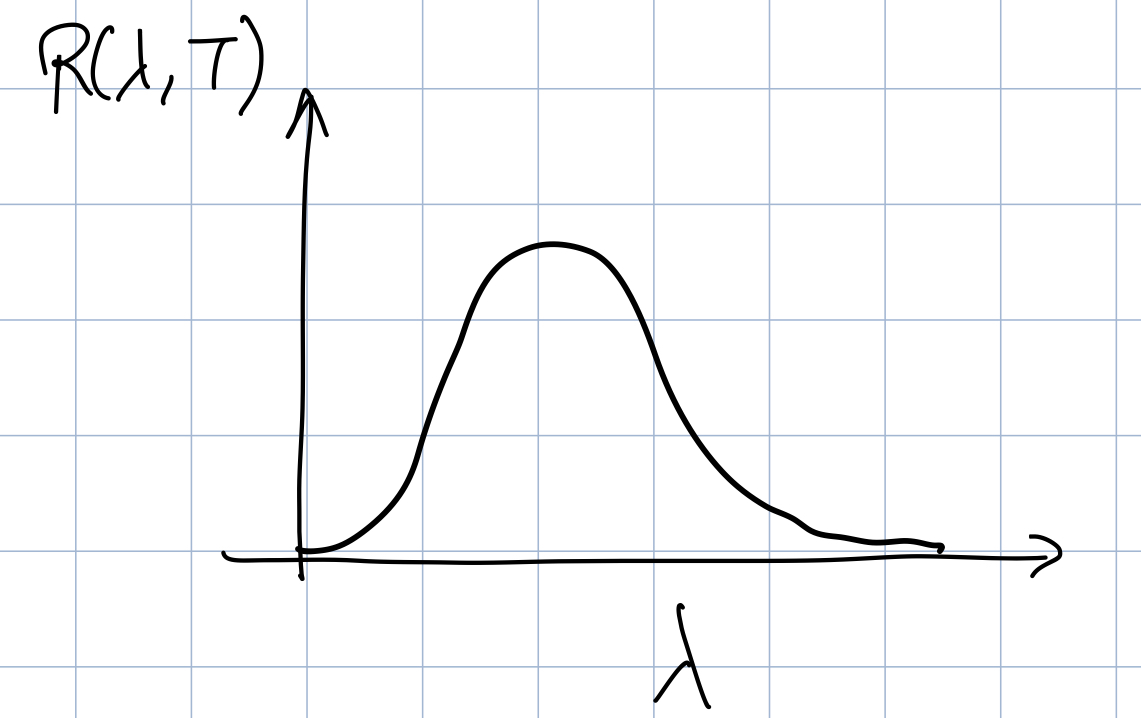
\includegraphics[width=200px]{../images/Kirchoff_model.jpeg}
    \end{center}
    The idea is that there are multiple collisions between the walls and the radiation field. The blackbody (as a perfect absorber) is absorbing all light at all frequencies.
    It looked something like this. The left-side is near 0 because you have no wave at that wavelength. The right side must be bounded because we want total emissive power to be finite (or do we?).
    \item 1879: Stefan's Law
    \[ \int_{0}^{\infty} R(\lambda, T) \dd{\lambda} = \sigma T^4 \]
    i.e. the total radiation emitted is proportional to $T^4$, which $\sigma \approx 5.67 \times 10^{-8} \frac{W}{m^2 K^4}$ 
    \item ????: Wien's Law
    \[ \lambda_{max} T \approxeq 2.898 \times 10^{-3} m \cdot K\]
    i.e. these curves all have the same constant for the quantity. For example, in the following graph, $T_1 > T_2$.
    \begin{center}
        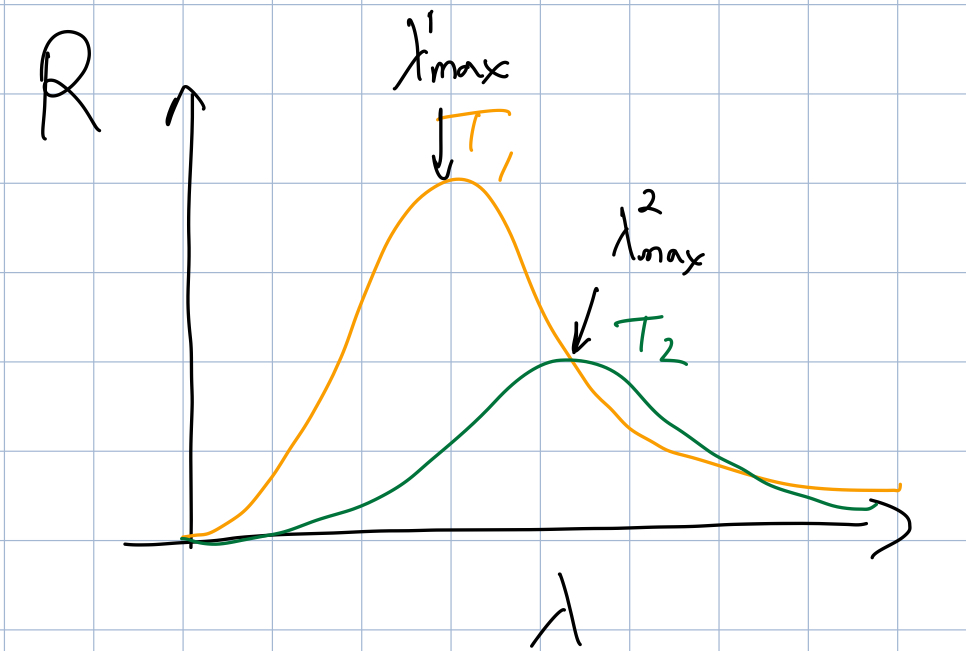
\includegraphics[width=200px]{../images/Wiens_law.jpeg}
    \end{center}
    \item ????: Rayleigh-Jeans Law
    \[ R(\lambda, T) \propto \frac{8 \pi k_B T}{\lambda^4} \]
    which only works at longer frequencies (the area is unbounded). The original derivation was similar to many observations in astronomy (guess a power law and add fudge factors).
\end{itemize}

\subsection{A Formal Derivation}

Let's derive the last law using thermodynamic principles and waves. We will analyze the energy density that the light trapped in the solid
produces. The energy of a light wave increases with frequency, which in turn is proportional to the number of wave modes. In other words:
\[ \text{Energy} = \text{Number of modes} \times \text{Energy per mode} \]
Suppose our blackbody is a cube of length $L$.
\begin{center}
    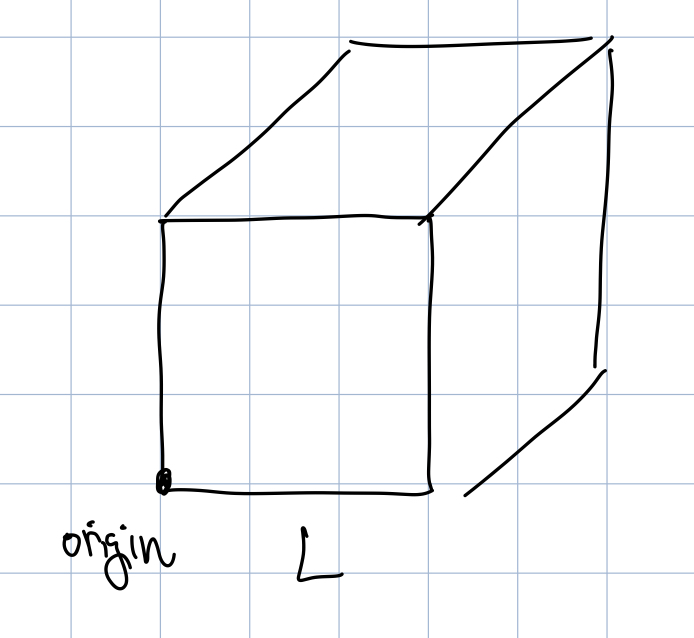
\includegraphics[width=200px]{../images/L_cube.jpeg}
\end{center}
Let's find the waves that are stable in the cube.
First, we write the wave equation.
\[ \nabla^2 \Psi(\mbf{r}, t) = \frac{1}{c^2} \partialderivative{^2}{t^2} \Psi(\mbf{r}, t) \]
where
\[ \nabla^2 = \partialderivative{^2}{x^2} + \partialderivative{^2}{y^2} + \partialderivative{^2}{z^2} \]

In addition, we need boundary conditions--consider a standing wave in 1-d. At the ends it is fixed at 0. For 3-d this is:
\begin{align*}
    \Psi(x = 0, y, z, t) &= \Psi(x = L, y, z, t) = 0, \forall y, z, t \\ 
    \Psi(x, y = 0, z, t) &= \Psi(x, y = L, z, t) = 0, \forall x, z, t \\
    \Psi(x, y, z = 0, t) &= \Psi(x, y, z = L, t) = 0, \forall x, y, t
\end{align*}

The solution is:
\[ \Psi(\mbf{r}, t) = A(t) \sin(k_x x) \sin(k_y y) \sin(k_z z) \]
where $k_i = \frac{n_i \pi }{L}$ for $n_i \in \N$. $n_i$ is the number of nodes along the $i$th axis. Each tuple of $n_i$ is a valid mode (configuration) of the wave.

This looks like:
\[ \Psi(\mbf{r}, t) = A(t) B(x, y, z) \]
So we are modulating the space component of the wave with some $A(t)$ that changes over the time. This is true for any standing wave.